\documentclass[11pt, french, english]{article}

\input{../common/modules}
\input{../common/commands}
\input{../common/macros_guillaume}

\usepackage{cancel}
\usepackage{aligned-overset}

%%%%%%%%% STUDENTS CHANGE THIS

\providetoggle{undergrad}
\settoggle{undergrad}{true}     %%% "true" if 3395 or "false" if 6390

\providetoggle{french}
\settoggle{french}{true}        %%% "true" if french or "false" if english

\providetoggle{final}            
\settoggle{final}{true}        %%% "true" for your final homework submission (removes instructions)

%%%%%%%%%%%%%%%%%%%%% ^^^^^


\begin{document}

\setlength{\parskip}{0.3cm} \setlength{\parindent}{0cm}

\begin{center}
	\textbf{IFT-3395 Fundamentals of Machine Learning} \\
	\textbf{Professor: Guillaume Rabusseau }
	\par\end{center}{\large \par}

\begin{center}
	\textbf{\LARGE{\enfr{Homework 2 - Theoretical part}{Devoir 2 - Partie Th\'eorique}}} \\
	\par\end{center}{\LARGE \par}
	
Mathis Koroglu : 20223045\\
Antonin Roy : 20145595

\instruct{
	\begin{itemize}
		\item
		      \enfr{
			      This homework must be done and submitted to Gradescope and can be done  \iftoggle{undergrad}{in groups of up to 3}{in groups of up to 2} students.
			      You are welcome to discuss with students outside of your group  \emph{but the solution submitted by a group must be its own}.
			      Note that we will use Gradescope's plagiarism detection feature.
			      All suspected cases of plagiarism will be recorded and shared with university officials for further handling.\\
		      }{
			      Ce devoir doit être déposé sur Gradescope  et peut-être être fait \iftoggle{undergrad}{en groupe jusqu'à 3}{en groupe jusqu'à 2} étudiants. Vous pouvez discuter avec des étudiants d'autres groupes  \emph{mais les réponses soumises par le groupe doivent être originales}. A noter que nous utiliserons l'outil de détection de plagiat de Gradescope. Tous les cas suspectés de plagiat seront enregistrés et transmis à l'Université pour vérification.
		      }

		\item
		      \enfr{
			      \emph{Only one student should submit the homework} and you should add your group member on the submission page on Gradescope.
		      }{
			      \emph{Un seul étudiant doit soumettre les solutions} et vous devez ajouter votre membre d'équipe sur la page de soumission de Gradescope.
		      }
		      % \item 
		      % \enfr{
		      % You need to submit your solution as a pdf file on Gradescope using the homework titled 
		      % \iftoggle{undergrad}{\texttt{(3395: UNDERGRAD) Homework 3}}{\texttt{(6390: GRAD) Homework 2 Theory}}.
		      % }{
		      % Vous devez soumettre vos solutions au format pdf sur Gradescope en utilisant le devoir intitulé \iftoggle{undergrad}{\texttt{(3395: UNDERGRAD) Homework 2 Theory}}{\texttt{(6390: GRAD) Homework 2 Theory}}.
		      % }\\
	\end{itemize}
}

\begin{enumerate}
	\item  \textbf{\enfr{Bias-Variance decomposition}{Décomposition biais/variance}}
\points{5 points}{5 points}

\enfr{
Consider the following data generation process: an input point $x$ is drawn from an unknown distribution and the output $y$ is generated using the formula
$$
	y = f(x) + \epsilon,
$$
where $f$ is an unknown deterministic function and $\epsilon \sim \mathcal{N}(0,\,\sigma^{2})$. This  process implicitly defines a distribution over inputs and outputs; we denote this distribution by $p$.

Given an i.i.d. training dataset $D=\{({x}_1, y_1),\dots,({x}_n, y_n)\}$ drawn from $p$, we can fit the hypothesis $h_D$ that minimizes the empirical risk with the squared error loss function. More formally,
$$
	h_D= \argmin_{h\in \mathcal H}  \sum_{i=1}^n (y_i - h({x}_i))^2
$$
where $\mathcal H$ is the set of hypotheses (or function class) in which we look for the best hypothesis/function.

The expected error\footnote{Here the expectation is over random draws of the training set $D$ of $n$ points from the unknown distribution $p$. For example (and more formally): $\Esp[(h_D({x'})] = \Esp_{(x_1,y_1)\sim p} \cdots \Esp_{(x_n,y_n)\sim p} \Esp[(h_{\{({x}_1, y_1),\dots,({x}_n, y_n)\}}({x'})]$.}  of $h_D$ on a fixed data point $(x',y')$ is given by $\Esp[(h_D({x'}) - y')^2]$. Two meaningful terms that can be defined are:
\begin{itemize}
	\item The \emph{bias}, which is the difference between the expected value of hypotheses at ${ x}'$ and the true value  $f({x'})$. Formally,
	      $$
		      \textit{bias}= \Esp[h_D({x'})]-f({x'})
	      $$
	\item The \emph{variance}, which is how far hypotheses learned on different datasets are spread out from their mean $\Esp[h_D({x'})]$. Formally,
	      $$
		      \textit{variance}= \Esp[(h_D({x'}) - \Esp[h_D({x'})])^2]
	      $$
\end{itemize}

Show that the expected prediction error on $({x'},y')$ can be decomposed into a sum of 3 terms: $(\textit{bias})^2$, $\textit{variance}$, and a $\textit{noise}$ term involving $\epsilon$. You need to justify all the steps in your derivation.

}{

Considérons les données générées de la manière suivante: une donnée $x$ est échantillonnée à partir d'une distribution inconnue, et nous observons la mesure correspondante $y$ générée d'après la formule
$$
	y = f(x) + \epsilon,
$$
où $f$ est une fonction déterministe inconnue et  $\epsilon \sim \mathcal{N}(0,\,\sigma^{2})$. Ceci définit une distribution sur les données $x$ et mesures $y$, nous notons cette distribution $p$.

Étant donné un ensemble d'entraînement $D=\{({x}_1, y_1),\dots,({x}_n, y_n)\}$ échantillonné i.i.d. à partir de $p$, on définit l'hypothèse $h_D$ qui minimise le risque empirique donné par la fonction de coût erreur quadratique. Plus précisément,
$$
	h_D= \argmin_{h\in \mathcal H}  \sum_{i=1}^n (y_i - h({x}_i))^2
$$
où $\mathcal H$ est l'ensemble d'hypothèses (ou classe de fonction) dans lequel nous cherchons la meilleure fonction/hypothèse.

L'erreur espérée\footnote{Ici l'espérance porte sur le choix aléatoire d'un ensemble d'entraînement $D$ de $n$ points tirés à partir de la distribution inconnue $p$. Par exemple (et plus formellement) : $\Esp[(h_D({x'})] = \Esp_{(x_1,y_1)\sim p} \cdots \Esp_{(x_n,y_n)\sim p} \Esp[(h_{\{({x}_1, y_1),\dots,({x}_n, y_n)\}}({x'})]$.} de $h_D$ sur un point donné $(x^{\prime}, y^{\prime})$ est notée $\Esp_{D \sim p^n} \left[\left(h_{D}(x^{\prime}) - y^{\prime}\right)^{2}\right]$. Deux termes importants qui peuvent être définis sont:
\begin{itemize}
	\item Le \emph{biais}, qui est la différence entre l'espérance de la valeur donnée par notre hypothèse en un point ${ x}'$ et la vraie valeur donnée par  $f({x'})$. Plus précisément,
	      $$
		      \textit{biais}= \Esp_{D \sim p^n}\left[h_D({x^{\prime}})\right]-f({x^{\prime}})
	      $$
	\item La \emph{variance}, est une mesure de la dispersion des hypothèse apprises sur des ensemble de données différents, autour de la moyenne $\Esp_{D \sim p^n}\left[h_D({x^{\prime}})\right]$. Plus précisément,
	      $$
		      \textit{variance}= \Esp_{D \sim p^n}\left[(h_D({x^{\prime}}) - \Esp_{D \sim p^n}\left[h_D({x^{\prime}})\right])^2\right]
	      $$
\end{itemize}

Montrez que l'erreur espérée pour un point donné $({x^{\prime}},y^{\prime})$ peut être décomposée en une somme de 3 termes: $(\textit{biais})^2$, $\textit{variance}$, et un terme de $\textit{bruit}$ qui contient $\epsilon$. Vous devez justifier toutes les étapes de dérivation.
}

\newpage

\begin{reponse}

	Rappelons que $\Esp\left[\Esp\left[u\right]\right]= \Esp\left[u\right]$

	\begin{align*}
		\Esp\left[\left(h_D\left({x^{\prime}}\right) - y^{\prime}\right)^2\right]
		 & = \Esp\left[\left(h_D\left({x^{\prime}}\right) - f\left(x^{\prime}\right)+f\left(x^{\prime}\right)- y^{\prime}\right)^2\right]         \\
		 & = \Esp\left[\left(h_D\left({x^{\prime}}\right) - f\left(x^{\prime}\right)\right)^2\right]
		+ \Esp\left[\left(f\left(x^{\prime}\right)- y^{\prime}\right)^2\right]
		+ 2\Esp\left[\left(h_D\left({x^{\prime}}\right) - f\left(x^{\prime}\right)\right)\left(f\left(x^{\prime}\right)- y^{\prime}\right)\right] \\
	\end{align*}

	avec $\Esp\left[\left(f\left(x^{\prime}\right)- y^{\prime}\right)^2\right] = \Esp\left[\left(f\left(x^{\prime}\right) - \left(f\left(x^{\prime}\right) + \varepsilon\right)\right)^2\right] = \Esp\left[\varepsilon^2\right]$ et par linéarité de l'espérance :
	$$\Esp\left[\left(h_D\left({x^{\prime}}\right) - f\left(x^{\prime}\right)\right)\left(f\left(x^{\prime}\right)- y^{\prime}\right)\right] =
		\Esp\left[h_D\left({x^{\prime}}\right)f\left(x^{\prime}\right)\right]
		- \Esp\left[h_D\left({x^{\prime}}\right)y^{\prime}\right]
		- \Esp\left[f\left(x^{\prime}\right)^{2}\right]
		+ \Esp\left[f\left(x^{\prime}\right)y^{\prime}\right]$$

	Notons que :
	\begin{itemize}
		\item Comme $f$ est déterministe $\Esp\left[f\left(x^{\prime}\right)y^{\prime}\right] = f\left(x^{\prime}\right)\Esp\left[y^{\prime}\right] = f\left(x^{\prime}\right)^2$
		      \\puisque $\Esp\left[y^{\prime}\right] = \Esp\left[f\left(x^{\prime}\right) + \varepsilon\right]= f\left(x^{\prime}\right)$
		      car ($\Esp\left[\varepsilon\right]=0$)
		\item $\Esp\left[f\left(x^{\prime}\right)^{2}\right] = f\left(x^{\prime}\right)^{2}$ car $f$ est déterministe
		\item $\Esp\left[h_D\left({x^{\prime}}\right)y^{\prime}\right] = \Esp\left[h_D\left({x^{\prime}}\right)\left(f\left(x^{\prime}\right) + \varepsilon\right)\right] = \Esp\left[h_D\left({x^{\prime}}\right)f\left(x^{\prime}\right) + h_D\left({x^{\prime}}\right)\varepsilon\right] = \Esp\left[h_D\left({x^{\prime}}\right)f\left(x^{\prime}\right)\right]$ \\car $\Esp\left[h_D\left({x^{\prime}}\right)\varepsilon\right] = 0$, en effet notre hypothèse $h_D$ est indépendante du bruit, dont l'espérance vaut $0$
	\end{itemize}

	\begin{align*}
		\Esp\left[\left(h_D\left({x^{\prime}}\right) - f\left(x^{\prime}\right)\right)\left(f\left(x^{\prime}\right)- y^{\prime}\right)\right]
		 & =
		\Esp\left[h_D\left({x^{\prime}}\right)f\left(x^{\prime}\right)\right]
		- \Esp\left[h_D\left({x^{\prime}}\right)y^{\prime}\right]
		- \Esp\left[f\left(x^{\prime}\right)^{2}\right]
		+ \Esp\left[f\left(x^{\prime}\right)y^{\prime}\right]                      \\
		 & = \Esp\left[h_D\left({x^{\prime}}\right)f\left(x^{\prime}\right)\right]
		- \Esp\left[h_D\left({x^{\prime}}\right)f\left(x^{\prime}\right)\right]
		- f\left(x^{\prime}\right)^{2}
		+ f\left(x^{\prime}\right)^{2}                                             \\
		 & = 0
	\end{align*}

	D'où :
	$$\Esp\left[\left(h_D\left({x^{\prime}}\right) - y^{\prime}\right)^2\right]
		= \Esp\left[\left(h_D\left({x^{\prime}}\right) - f\left(x^{\prime}\right)\right)^2\right]
		+ \Esp\left[\varepsilon^2\right]$$

	\begin{align*}
		\Esp\left[\left(h_D\left({x^{\prime}}\right) - f\left(x^{\prime}\right)\right)^2\right]
		=  & \Esp\left[\left(h_D\left({x^{\prime}}\right) - \Esp\left[h_D\left({x^{\prime}}\right)\right]+\Esp\left[h_D\left({x^{\prime}}\right)\right]-f\left(x^{\prime}\right)\right)^2\right]               \\
		=  & \underbrace{\Esp\left[\left(h_D\left({x^{\prime}}\right) - \Esp\left[h_D\left({x^{\prime}}\right)\right]\right)^2\right]}_{variance}
		+ \Esp\left[\left(\Esp\left[h_D\left({x^{\prime}}\right)\right]-f\left(x^{\prime}\right)\right)^2\right]                                                                                               \\
		{} & + 2 \Esp\left[\left(h_D\left({x^{\prime}}\right) - \Esp\left[h_D\left({x^{\prime}}\right)\right]\right)\left(\Esp\left[h_D\left({x^{\prime}}\right)\right]-f\left(x^{\prime}\right)\right)\right]
	\end{align*}

	Comme $f$ est déterministe $\Esp\left[f\left(x^{\prime}\right)\right] = f\left(x^{\prime}\right)$ et $\operatorname{Var}\left(f\right) = 0$, d'où :
	\begin{align*}
		\Esp\left[\left(\Esp\left[h_D\left({x^{\prime}}\right)\right]-f\left(x^{\prime}\right)\right)^2\right]
		 & = \Esp\left[\Esp\left[h_D\left({x^{\prime}}\right)\right]-f\left(x^{\prime}\right)\right]^2
		+ \operatorname{Var}\left(\Esp\left[h_D\left({x^{\prime}}\right)\right]-f\left(x^{\prime}\right)\right)                                                                                                 \\
		 & = \left(\Esp\left[\Esp\left[h_D\left({x^{\prime}}\right)\right]\right]-\Esp\left[f\left(x^{\prime}\right)\right]\right)^2 + \underbrace{\operatorname{Var}\left(f\left(x^{\prime}\right)\right)}_{0} \\
		 & = \left(\Esp\left[h_D\left({x^{\prime}}\right)\right]-f\left(x^{\prime}\right)\right)^2                                                                                                              \\
		 & = biais
	\end{align*}

	\begin{align*}
		\Esp\left[\left(h_D\left({x^{\prime}}\right) - \Esp\left[h_D\left({x^{\prime}}\right)\right]\right)\left(\Esp\left[h_D\left({x^{\prime}}\right)\right]-f\left(x^{\prime}\right)\right)\right]
		=  & \underbrace{\Esp\left[h_D\left({x^{\prime}}\right)\Esp\left[h_D\left({x^{\prime}}\right)\right]\right]}_{\Esp\left[h_D\left({x^{\prime}}\right)\right]^{2}}
		-\underbrace{\Esp\left[\Esp\left[h_D\left({x^{\prime}}\right)\right]^{2}\right]}_{\Esp\left[h_D\left({x^{\prime}}\right)\right]^{2}}                                                                                                                                                                     \\
		{} & +\underbrace{\Esp\left[\Esp\left[h_D\left({x^{\prime}}\right)\right]f\left(x^{\prime}\right)\right]}_{\underbrace{\Esp\left[f\left(x^{\prime}\right)\right]\Esp\left[\Esp\left[h_D\left({x^{\prime}}\right)\right]\right]}_{f\left(x^{\prime}\right)\Esp\left[h_D\left({x^{\prime}}\right)\right]}}
		- \underbrace{\Esp\left[h_D\left({x^{\prime}}\right) f\left(x^{\prime}\right)\right]}_{\underbrace{\Esp\left[f\left(x^{\prime}\right)\right]\Esp\left[h_D\left({x^{\prime}}\right)\right]}_{f\left(x^{\prime}\right)\Esp\left[h_D\left({x^{\prime}}\right)\right]}}                                      \\
		=  & 0
	\end{align*}

	Car $\operatorname{Cov}\left(f\left(x^{\prime}\right), h_D\left({x^{\prime}}\right)\right)=0$, étant donné que $f\left(x^{\prime}\right)$ est ici constant pour un $x$ donné

	En regroupant tous les termes on obtient :
	\begin{align*}
		\Esp\left[\left(h_D\left({x^{\prime}}\right) - y^{\prime}\right)^2\right]
		 & = biais + variance + \Esp\left[\varepsilon^2\right]
	\end{align*}

	avec $\Esp\left[\varepsilon^{2}\right]
		= \operatorname{Var}[\varepsilon]+\underbrace{\Esp\left[\varepsilon\right]^{2}}_{0} = \operatorname{Var}[\varepsilon] = \sigma^2$
\end{reponse}

	\item{
            \textbf{\enfr{ Feature Maps}{ Fonctions de transformation des données}}
            \points{10 points}{8 points}

            \enfr{
	            In this exercise, you will design feature maps to transform an original dataset into a linearly separable set of points. For the following questions, if your answer is `\textit{yes}', write the expression for the proposed transformation; and if your answer is `\textit{no}', write a brief explanation. You are expected to provide explicit formulas for the feature maps, and these formulas should only use common mathematical operations.
            }{
	            Dans cet exercice, vous allez concevoir des fonctions de transformation depuis l'espace de features original vers un espace où les données sont linéairement séparables. Pour les questions suivantes, si vous répondez `\textit{oui}', écrivez l'expression de la transformation correspondante; et si votre réponse est `\textit{non}', ajoutez une courte justification de votre réponse. Vous devez donner les formules explicites des transformations, et ces formules doivent utiliser uniquement des opérations mathématiques simples.
            }

            \begin{enumerate}
	            \item { [3 points] \enfr{
		                  Consider the following 1-D dataset (Figure \ref{a}). Can you propose a 1-D transformation that will make the points linearly separable?
	                  }{
		                  Soient les données 1-D suivantes (Figure \ref{a}). Pouvez-vous proposer une transformation 1-D (i.e. vers un espace de dimension 1) qui rend les points linéairement séparables?
	                  }

	                  \begin{figure}[!h]
		                  \centering
		                  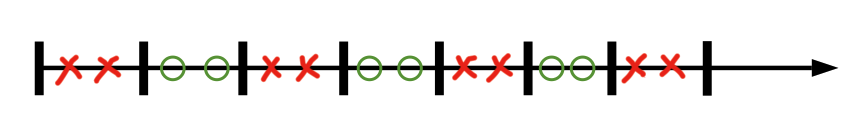
\includegraphics[width=0.55\textwidth]{img/Q2-a.png}
		                  \caption{\enfr{1-D dataset. The points between $2k$ and $2k+1$ are labeled by X. The points between $2k+1$ and $2k+2$ are labeled by O.}{Jeu de données 1D. Les points entre $2k$ et $2k+1$ sont étiquetés par X. Les points entre $2k+1$ et $2k+2$ sont étiquetés par O.}}
		                  \label{a}
	                  \end{figure}}
	                  %     \item {[2 points] In the same dataset, can you propose a 2-D transformation that makes the points linearly separable?}

	                  \begin{reponse}

		                  La transformation 1-D suivante sépare linéairement les points étiquetés par X et O :
		                  \begin{equation*}
			                  \phi(x) = \sin\left(\pi x\right)
		                  \end{equation*}
		                  $\phi(x) \geq 0$ lorsque $x \in$X et $\phi(x) < 0$ si $x \in$O
	                  \end{reponse}

	            \item { [3 points]
	                  \enfr{
		                  Consider the following 2-D dataset (Figure \ref{b}). Can you propose a transformation into 1-D that will make the data linearly separable?
	                  }{
		                  Soient les données 2-D suivantes (Figure \ref{b}). Pouvez-vous proposer une transformation 1-D qui rend les points linéairement séparables ?
	                  }
	                  \begin{figure}[h]
		                  \centerline{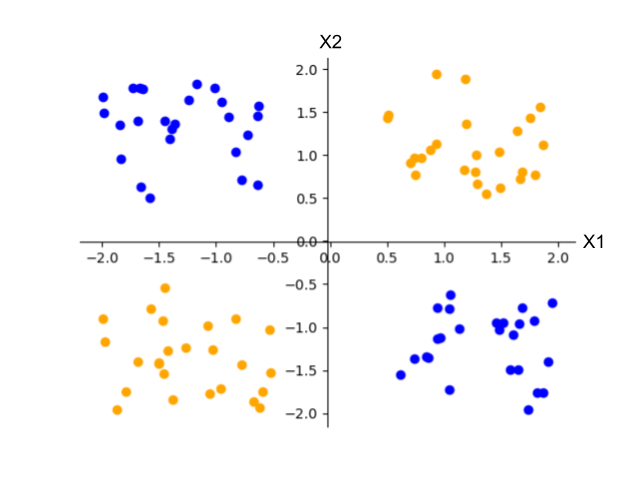
\includegraphics[scale=0.4]{img/Q2-b.png}}
		                  \caption{\enfr{2D dataset.}{Jeu de données 2D.}}
		                  \label{b}
	                  \end{figure}}

	                  \begin{reponse}

		                  La transformation 1-D suivante sépare linéairement les points bleus et orange :

		                  Soit $x\in \mathbb{R}^2$
		                  \begin{equation*}
			                  \phi\left(x\right)
			                  = \phi\left( \begin{bmatrix}
					                  x_1 \\
					                  x_2\end{bmatrix}\right) = x_1 x_2 \in \mathbb{R}
		                  \end{equation*}
		                  $\phi(x) \geq 0$ lorsque $x$ est un point appartenant à la classe orange et $\phi(x) < 0$ si $x$ est dans la classe bleue
	                  \end{reponse}

	            \item { [4 points]
	                  \enfr{
		                  Using ideas from the above two datasets, can you suggest a transformation of the following dataset (as shown in Figure \ref{12}) that makes it linearly separable? If `\textit{yes}', also provide the kernel corresponding to the feature map you proposed. Remember that $K(x, y)=\phi(x) \cdot \phi(y)$, so you can find $\phi$ and do the dot product to find an expression for the kernel.
	                  }{
		                  En utilisant les idées que vous avez utilisées pour les deux questions précédentes, pouvez-vous proposer une transformation des données suivantes (Figure \ref{12}) qui les rendent linéairement séparables? Si votre réponse est `\textit{oui}', donnez l'expression du noyau qui correspond à la transformation proposée. Souvenez-vous que $K(x, y)=\langle\phi(x) , \phi(y)\rangle$, donc trouvez $\phi$ et faites le produit scalaire pour obtenir le noyau.
	                  }
	                  \begin{figure}[H]
		                  \centering
		                  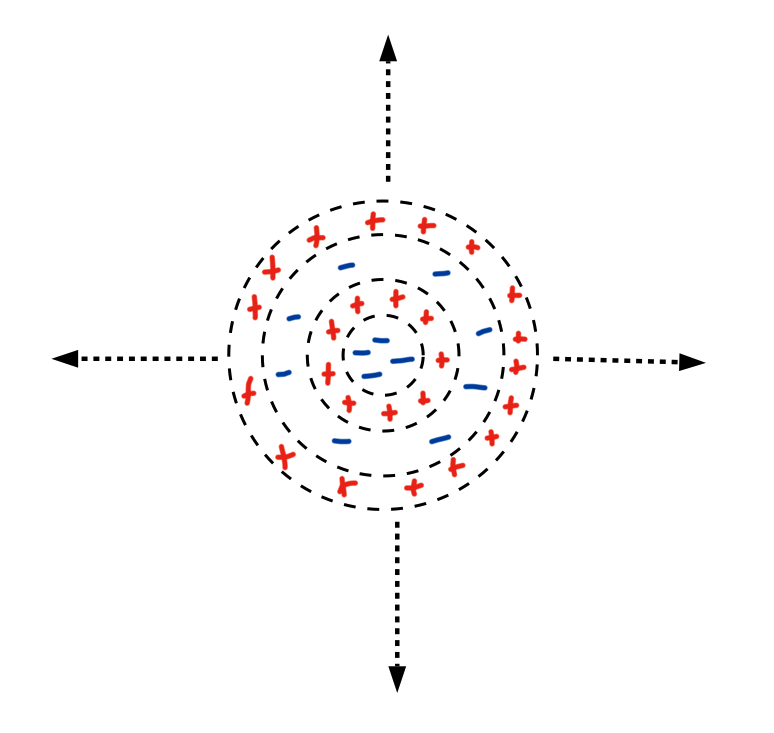
\includegraphics[scale=0.5]{img/Q2-c.png}
		                  \caption{\enfr{Another 2D dataset. The points between the areas of radius $2k$ and $2k+1$ are labeled by -. The points between the areas of radius $2k+1$ and $2k+2$ are labeled by +.}{Un autre jeu de données 2D. Les points entre les aires de rayon $2k$ et $2k+1$ sont étiquetés par -. Les points entre les aires de rayon $2k+1$ et $2k+2$ sont étiquetés par +.}}
		                  \label{12}
	                  \end{figure}}

	                  \begin{reponse}

		                  La transformation 3-D suivante sépare linéairement les points appartenant aux classes "+" et "-" selon le plan $z=0$

		                  Soit $x\in \mathbb{R}^2$
		                  \begin{equation*}
			                  \phi\left(x\right)
			                  = \phi\left( \begin{bmatrix}
					                  x_1 \\
					                  x_2\end{bmatrix}\right) = \begin{bmatrix}
				                  x_1 \\
				                  x_2 \\
				                  \sin\left(\pi {\lVert x \rVert}_2 \right)\end{bmatrix} \in \mathbb{R}^3
		                  \end{equation*}

		                  Déterminons maintenant le noyau :
		                  \begin{align*}
			                  K(x, y)
			                   & = \langle\phi(x),\phi(y)\rangle                                                                       \\
			                   & = x_1 y_1 + x_2 y_2 + \sin\left(\pi{\lVert x \rVert}_2\right)\sin\left(\pi{\lVert y \rVert}_2\right)  \\
			                   & = \langle x,y\rangle + \sin\left(\pi{\lVert x \rVert}_2\right)\sin\left(\pi{\lVert y \rVert}_2\right)
		                  \end{align*}

		                  \underline{Remarque :} On pourrait se contenter de la transformation 1-D : $\phi\left(x\right) = \sin\left(\pi {\lVert x \rVert}_2 \right)$
	                  \end{reponse}

            \end{enumerate}
      }

	%\item \textbf{\enfr{Derivatives and Gradients }{Dérivés et gradients}}
\points{IFT6390 - Non demandé}{14 points}

\enfr{In this question, we will look at derivatives and gradients. Chapter 5 of Mathematics for Machine Learning book can be used as reference for this question.}{Dans cette question, nous examinerons les dérivées et les gradients. Le Chapitre 5 de ``Mathematics for Machine Learning'' peut être utilisé comme référence pour cette question.}

\begin{enumerate}
	\item{[2 points] \enfr{
		            Compute the derivative $f^{'}\left(x\right)$ for:\\
		            $$f\left(x\right)=\log\left(x^4\right)\sin\left(x^3\right)$$\\
	            }
	            {Calculer la dérivée $f^{'}\left(x\right)$ pour: \\
		            $$f\left(x\right)=\log\left(x^4\right)\sin\left(x^3\right)$$\\}
	      }
	      
	      \begin{reponse}
	      	\begin{align*}
	      		f^{'}\left(x\right)
	      		&= \log\left(x^4\right)^\prime \sin\left(x^3\right) + \sin\left(x^3\right)^\prime \log\left(x^4\right)\\
	      		&= \frac{4}{x} \sin\left(x^3\right) + 3x^2\cos\left(x^3\right)\log\left(x^4\right)
	      	\end{align*}
	      \end{reponse}

	\item { [2 points] \enfr{Compute the derivative $f^{'}\left(x\right)$ for:\\
		      $$f\left(x\right)=\exp\left(\frac{-1}{2\sigma }\left(x-\mu \right)^2\right)$$
		      Here $\sigma$,$\mu$ $\in \mathbb{R}$.\\~\\
	      }
	      { Calculer la dérivée $f^{'}\left(x\right)$ pour:\\ $$f\left(x\right)=\exp\left(\frac{-1}{2\sigma }\left(x-\mu \right)^2\right)$$
		      où $\sigma,\mu \in \mathbb{R}.$\\~\\}
	      }
	      
	      \begin{reponse}
	      	\begin{align*}
	      		f^{'}\left(x\right)
	      		&= \left(\frac{-1}{2\sigma }\left(x-\mu \right)^2\right)^\prime \exp\left(\frac{-1}{2\sigma }\left(x-\mu \right)^2\right)\\
	      		&= \frac{-1}{2\sigma } 2 \left(x -\mu \right) \exp\left(\frac{-1}{2\sigma }\left(x-\mu \right)^2\right)\\
	      		&= \frac{\mu-x}{\sigma} \exp\left(\frac{-1}{2\sigma }\left(x-\mu \right)^2\right)
	      	\end{align*}
	      \end{reponse}

	\item { [4 points] \enfr{Consider the following functions:\\
		      $$f_1\left(x\right)=\sin\left(x_1\right)\cos\left(x_2\right), \:x\:\in \:\mathbb{R}^2$$
		      $$f_2\left(x,y\right)=x^Ty\:$$
		      Here $\:x,y\:\in \:\mathbb{R}^n$.\\
		      $$f_3\left(x\right)=xx^T\:$$
		      Here $\:x\:\in \:\mathbb{R}^n$.\\~\\
		      i. What are the dimensions of $\frac{\partial f_i}{\partial x}$?\\
		      ii. Compute the jacobians.\\~\\

	      }{Considérez les fonctions suivantes:\\
		      $$f_1\left(x\right)=\sin\left(x_1\right)\cos\left(x_2\right), \:x\:\in \:\mathbb{R}^2$$
		      $$f_2\left(x, y\right)=x^{\top}y\:$$
		      Ici $\:x,y\:\in \:\mathbb{R}^n$.\\
		      $$f_3\left(x\right)=xx^\top\:$$
		      Ici $\:x\:\in \:\mathbb{R}^n$.\\~\\
		      i. Quelles sont les dimensions de $\frac{\partial f_i}{\partial x}$?\\
		      ii. Calculer le jacobien.\\~\\}
	      }

	\item { [6 points] \enfr{Compute the derivatives $\frac{df}{dx}$ of the following functions:\\
	      i. Use the chain rule. Provide the dimensions of every derivative.\\
	      $$f\left(z\right)=exp\left(-\frac{1}{2}z\right)$$
	      $$z=g\left(y\right)=y^TS^{-1}y$$
	      $$y=h\left(x\right)=x-\mu$$
	      Here $ x, \mu \in \mathbb{R}^D, S \in \mathbb{R}^{D \times D}$.\\~\\
	      ii. $$f\left(x\right)=tr\left(xx^{\top}+\sigma I\right)\:$$
	      Here $\:x\in \mathbb{R}^D$ and $tr\left(A\right)$ is the trace of A.\\~\\
	      iii. Use the chain rule to compute the derivatives and provide the dimensions of the partial derivative as well.\\
	      $$f=\tanh\left(z\right)$$
	      Here $f \in \mathbb{R}^M$.
	      $$z=Ax+b\:$$
	      Here $\:x\:\in \mathbb{R}^N,\:A\in \:\mathbb{R}^{M \times N}\:,\:b\:\in \:\mathbb{R}^M$.\\~\\

	      }
	      {Calculer les dérivées $\frac{df}{dx}$ des fonctions suivantes:\\
	      i. Utilisez la règle de la chaîne. Donnez les dimensions de chaque dérivée.\\
	      $$f\left(z\right)=\exp\left(-\frac{1}{2}z\right)$$
	      $$z=g\left(y\right)=y^{\top}S^{-1}y$$
	      $$y=h\left(x\right)=x-\mu$$
	      où $x, \mu \in \mathbb{R}^D, S \in \mathbb{R}^{D \times D}$.\\~\\
	      ii. $$f\left(x\right)=tr\left(xx^{\top}+\sigma I\right)\:$$
	      Ici $\:x\in \mathbb{R}^D$ and $tr\left(A\right)$ est la trace de A.\\~\\
	      iii. Utilisez la règle de la chaîne pour calculer les dérivées et fournir également les dimensions de la dérivée partielle.\\
	      $$f=\tanh\left(z\right)$$
	      Ici $f \in \mathbb{R}^M$.
	      $$z=Ax+b\:$$
	      Ici $\:x\:\in \mathbb{R}^N,\:A\in \:\mathbb{R}^{M \times N}\:,\:b\:\in \:\mathbb{R}^M$.\\~\\
	      }
	      }

\end{enumerate}
	\item \textbf{\enfr{Bayes Risk }{Risque de Bayes}}
\points{15 points}{10 points}

\newcommand{\lecture}[4]{
	\pagestyle{myheadings}
	\thispagestyle{plain}
	\newpage
	\setcounter{page}{1}
	\noindent
	\begin{center}
		\framebox{
			\vbox{\vspace{2mm}
				\hbox to 6.28in { {\bf ECE901 Spring 2007 Statistical Learning Theory \hfill Instructor: R. Nowak} }
				\vspace{6mm}
				\hbox to 6.28in { {\Large \hfill #1  \hfill} }
				\vspace{2mm}}
		}
	\end{center}
	\markboth{#1}{#1}
	\setlength{\headsep}{10mm}
	\vspace*{4mm}
}

%notation

\def\X{\ensuremath{{\mathcal X}}}
\def\Y{\ensuremath{{\mathcal Y}}}
\def\F{\ensuremath{{\mathcal F}}}
\def\R{\ensuremath{{\bf R}}}
\def\E{\mathbb{E}}
\def\sign{\ensuremath{\mbox{sign}}}
\def\ie{{\em i.e.,}}

\enfr{In this exercise, we will show that the Bayes classifier (assuming we use the true underlying target distribution) minimize the true risk over all possible classifiers.

	Recall that the goal of binary classification is to learn a mapping $f$ from the input space, $\X$, to to the class space, $\Y=\{0,1\}$.
	We can measure the loss of a classifier $f$ using the $0-1$ loss; \ie
	$$\ell(\hat{y},y) = \1{\hat{y}\neq y} = \left\{ \begin{array}{ll}
			1, \;\; & \text{if } \hat{y}\neq y \\
			0, \;\; & \text{otherwise}\end{array}
		\right.$$

	Recall that the true risk of $f$ is defined by
	$$R(f) = \E_{(x,y)\sim \mathcal{P}}\left[\ell(f(x),y)\right]$$
	where $\mathcal{P}$ is the underlying target distribution.

	Usually, we assume that $\mathcal{P}$ is unknown and we infer $f$ from a dataset drawn from $\mathcal{P}$. For this exercise, we will consider
	the Bayes classifier built using the target distribution $\mathcal{P}$, which is defined by
	$$f^{\star}(x) = \left\{ \begin{array}{ll}
			1,\;\; & \text{if }\eta(x) \geq 1/2 \\
			0,\;\; & otherwise\end{array}
		\right.$$
	where
	$\eta(x) \equiv P(Y=1 | X=x).$

	\medskip

	You will show that for any function $g:\X\to\Y$ we have $R(g) \geq R(f^{\star})$

	\begin{enumerate}
		\item First, show that $R(f) = P_{(x,y)\sim \mathcal{P}}(f(x)\neq y)$.
		\item Show that, for any $g:\X\to\Y$,
		      $$
			      P(g(x)\neq y \mid X=x)= 1- \left[ \1{g(x)=1}\eta(x) + \1{g(x)=0}\left(1-\eta(x)\right)
				      \right]$$
		\item Using the answer to the previous question, and the fact that $\1{g(x)=0}=1-\1{g(x)=1}$, show that, for any $g:\X\to\Y$,
		      $$P\left(g(x)\neq Y | X=x\right)-P\left(f^{\star}(x)\neq Y|X=x\right) = \left(2\eta(x)-1\right)\left(\1{f^{\star}(x)=1}-\1{g(x)=1}\right)
		      $$
		\item Finally, show that, for any $g:\X\to\Y$, $$ \left(2\eta(x)-1\right)\left(\1{f^{\star}(x)=1}-\1{g(x)=1}\right) \geq 0$$
		\item Conclude.
	\end{enumerate}
}
{
	Dans cet exercice, nous montrerons que le classificateur de Bayes (en supposant que nous utilisions la vraie distribution cible sous-jacente) minimise le risque réel sur tous les classificateurs possibles.

	Rappelons que le but de la classification binaire est d'apprendre une fonction $f$ de l'espace d'entrée, $\X$, vers l'espace des classes, $\Y=\{0,1\}$.
	On peut mesurer la qualité d'un classificateur $f$ en utilisant la fonction de coût $0-1$; \ie
	$$\ell(\hat{y},y) = \1{\hat{y}\neq y} = \left\{ \begin{array}{ll}
			1, \;\; & \text{if } \hat{y}\neq y \\
			0, \;\; & \text{otherwise}\end{array}
		\right.$$

	Rappelons que le vrai risque de $f$ est défini par
	$$R(f) = \E_{(x,y)\sim \mathcal{P}}\left[\ell(f(x),y)\right]$$
	où $\mathcal{P}$ est la distribution cible sous-jacente.

	Habituellement, nous supposons que $\mathcal{P}$ est inconnu et nous déduisons $f$ à partir d'un ensemble de données tirées de $\mathcal{P}$. Pour cet exercice, nous considérerons
	le classifieur de Bayes construit en utilisant la distribution cible $\mathcal{P}$, qui est définie par
	$$f^{\star}(x) = \left\{ \begin{array}{ll}
			1,\;\; & \text{si }\eta(x) \geq 1/2 \\
			0,\;\; & \text{sinon}\end{array}
		\right.$$
	où
	$\eta(x) \equiv P(Y=1 | X=x).$

	\medskip

	Vous montrerez que pour n'importe quelle fonction $g:\X\to\Y$ on a $R(g) \geq R(f^{\star})$

	\begin{enumerate}
		\item Tout d'abord, montrez que
		      \begin{equation} \label{eq:a} \tag{a}
			      R(f) = P_{(x,y)\sim \mathcal{P}}(f(x)\neq y)
		      \end{equation}

		      \begin{reponse}
			      \begin{align*}
				      R\left( f \right)
				       & =
				      \Esp_{(x,y) \sim \mathcal{P}}\left[\ell(f(x), y)\right]
				      \\
				       & =
				      \Esp_{(x,y) \sim \mathcal{P}}\left[\1{\hat{y} \neq y}\right]
				      \\
				       & =
				      \sum_{z \in \{0,1\}}\left(z \cdot P\left(\1{f(x) \neq y}\right) = z\right)
				      \\
				       & =
				      P\left(\1{f(x) \neq y } = 1 \right)
				      \\
				       & =
				      P_{\left(x,y\right) \sim \mathcal{P}}\left(f(x) \neq y)\right)
			      \end{align*}
		      \end{reponse}

		\item Montrez que, pour tout $g:\X\to\Y$,
		      \begin{equation} \label{eq:b} \tag{b}
			      P(g(x)\neq y \mid X=x)= 1- \left[ \1{g(x)=1}\eta(x) + \1{g(x)=0}\left(1-\eta(x)\right)
				      \right]
		      \end{equation}

		      \begin{reponse}
			      sachant que:
			      \begin{equation} \label{eq:*} \tag{*}
				      \Esp_{(x, y) \sim \mathcal{P}}\left[\1{f(x) \neq y}\right] = P\left(f(x) = y\right)
			      \end{equation}
			      On a:
			      \begin{align*}
				      P\left(g(x) \neq y \mid X = x\right)
				                                        & = 1 - P(g(x) = y \mid X = x)                                                                                                              \\
				                                        & = 1 - \left(P(Y = 1, g(x) = 1 \mid X = x\right) + P\left(Y = 0, g(x) = 0 \mid X = x)\right)                                               \\
				      \overset{\ref{eq:*}}              & {=} 1 - (\Esp\left[\1{y = 1} \cdot \1{g(x) = 1} \mid X = x\right] +\Esp\left[\1{y = 0} \cdot \1{g(x) = 0} \mid X = x\right])              \\
				      \overset{\text{indep}}            & {=}             1 - (\1{g(x) = 1} \cdot \Esp\left[\1{y = 1} \mid X = x\right] + \1{g(x) = 0} \cdot \Esp\left[\1{y = 0} \mid X = x\right]) \\
				      \overset{\ref{eq:*}}              & {=} 1 - ((\1{g(x) = 1} \cdot P(Y = 1 \mid X = x) + (\1{g(x) = 0} \cdot P(Y = 0 \mid X = x)))                                              \\
				      \overset{\Delta \text{ de } \eta} & {=} 1 - \left(\1{g(x) = 1} \cdot \eta(x) + \1{g(x) = 0} \cdot (1 - \eta(x)\right)
			      \end{align*}
		      \end{reponse}

		\item En utilisant la réponse à la question précédente et le fait que $\1{g(x)=0}=1-\1{g(x)=1}$, montrez que, pour toute fonction $g:\X\to\Y$,
		      \begin{equation} \label{eq:c}
			      \tag{c}
			      P\left(g(x)\neq Y | X=x\right)-P\left(f^{\star}(x)\neq Y|X=x\right) = \left(2\eta(x)-1\right)\left(\1{f^{\star}(x)=1}-\1{g(x)=1}\right)
		      \end{equation}

		      \begin{reponse}
			      En notant $a\left( x\right) = \1{g(x) = 1}$ et $b\left( x\right) = \1{f^{\star}(x) = 1}$
			      \begin{align*}
				         & P\left(g(x) \neq Y \mid X = x\right) - P\left(f^{\star}(x) \neq Y \mid X = x\right)                                                                                                                      \\
				      =  &
				      \left(1 - ((\1{g(x) = 1} \eta(x) + \1{g(x) = 0} (1 - \eta(x)))\right)-\left(1 - ((\1{f^{\star}(x) = 1} \eta(x) + \1{f^{\star}(x) = 0}(1 - \eta(x)))\right)                                                   \\
				      =  & \left(1 - ((\1{g(x) = 1} \eta(x) + (1 - \1{g(x) = 1}) (1 - \eta(x)))\right)                                                                                                                               \\
				      {} & -\left(1 - ((\1{f^{\star}(x) = 1} \eta(x) + (1 - \1{f^{\star}(x) = 1}) (1 - \eta(x)))\right)                                                                                                            \\
				      =  & \left(1 - (a\left( x\right) \eta + (1 - a\left( x\right))(1 - \eta\left(x\right)))\right)-\left(1 - (b\left( x\right) \eta\left(x\right) + (1 - b\left( x\right))(1 - \eta\left(x\right)))\right)         \\
				      =  & \left(1 - (a\left( x\right) \eta\left(x\right) + (1 - \eta\left(x\right) - a\left( x\right) + a\left( x\right) \eta\left(x\right)))\right)                                                                \\
				      {} & -\left(1 - (b\left( x\right) \eta\left(x\right) + (1 - \eta\left(x\right) - b\left( x\right) + b\left( x\right) \eta\left(x\right)))\right)                                                               \\
				      =  & \left(1 - (2 a\left( x\right) \eta\left(x\right) + 1 - \eta\left(x\right) - a\left( x\right))\right)-\left(1 - (2 b\left( x\right) \eta\left(x\right) + 1 - \eta\left(x\right) - b\left( x\right))\right) \\
				      =  & \left(-2 a\left( x\right) \eta\left(x\right) + \eta\left(x\right) + a\left( x\right)\right)-\left(-2 b\left( x\right) \eta\left(x\right) + \eta\left(x\right) + b\left( x\right)\right)                   \\
				      =  & 2 b\left( x\right) \eta\left(x\right) - 2 a\left( x\right) \eta\left(x\right) + b\left( x\right) -a\left( x\right)                                                                                        \\
				      =  & 2 \eta\left(x\right) (b\left( x\right) - a\left( x\right)) +\left(b\left( x\right)-a\left( x\right)\right)                                                                                                \\
				      =  & (2 \eta\left(x\right) - 1) (b\left( x\right) - a\left( x\right))                                                                                                                                          \\
				      =  & (2 \eta\left( x\right) - 1)(\1{f^{\star}(x) = 1} - \1{g(x) = 1})
			      \end{align*}
		      \end{reponse}

		\item Montrez que, pour tout $g:\X\to\Y$,
		      \begin{equation} \label{eq:d} \tag{d}
			      \left(2\eta(x)-1\right)\left(\1{f^{\star}(x)=1}-\1{g(x)=1}\right) \geq 0
		      \end{equation}

		      \begin{reponse}
			      Nous avons 2 cas :

			      \begin{itemize}
				      \item Si $\eta(x) \geq \frac{1}{2}$ :

				            Alors $\1{f^{\star}(x)=1} = \1{\eta(x) \geq \frac{1}{2}} = 1$ d'où

				            \begin{equation*}
					            \underbrace{(2 \eta(x)-1)}_{\geq 0} \underbrace{(\underbrace{\1{f^{\star}(x)=1}}_{1}-\underbrace{\1{g(x)=1}}_{0 \text{ ou } 1})}_{\geq 0} \geq 0
				            \end{equation*}

				      \item Si $\eta(x) < \frac{1}{2}$ :

				            Alors $\1{f^{\star}(x)=1} = \1{\eta(x) \geq \frac{1}{2}} = 0$ d'où
				            \begin{equation*}
					            \underbrace{(2 \eta(x)-1)}_{< 0} \underbrace{(\underbrace{\1{f^{\star}(x)=1}}_{0}-\underbrace{\1{g(x)=1}}_{0 \text{ ou } 1})}_{\leq 0} \geq 0
				            \end{equation*}
			      \end{itemize}

			      Pour tout $x$, on a donc $\left(2\eta(x)-1\right)\left(\1{f^{\star}(x)=1}-\1{g(x)=1}\right) \geq 0$
		      \end{reponse}

		\item Conclure.

		      \begin{reponse}
			      \begin{gather*}
				      \left(2\eta(x)-1\right)\left(\1{f^{\star}(x)=1}-\1{g(x)=1}\right) \geq 0\\
				      \overset{\ref{eq:c}}{\Leftrightarrow}\\
				      P\left(g(x)\neq Y | X=x\right)-P\left(f^{\star}(x)\neq Y|X=x\right) \geq 0\\
				      \Leftrightarrow\\
				      P\left(g(x)\neq Y | X=x\right) \geq P\left(f^{\star}(x)\neq Y|X=x\right)\\
				      \overset{\ref{eq:a}}{\Leftrightarrow}\\
				      R\left(g\right) \geq R\left(f^{\star}\right)
			      \end{gather*}
		      \end{reponse}

	\end{enumerate}
}

	\renewcommand{\X}{\mat{X}}
\newcommand{\hloo}[1]{h_{D\setminus #1}}
\newcommand{\simiid}{{\sim \atop \textit{iid}}}
\newcommand{\Hi}{\H_{ii}}

\item \textbf{\enfr{Leave one out cross-validation }{Validation croisée "leave-one-out"}}
\points{15 points}{10 points}

\enfr{
	Let $D = \{(x_1,y_1),\dots,(x_n,y_n)\}$ be a training sample set drawn i.i.d. from an unknown distribution $p$.
	Recall that leave-one-out cross-validation (LOO-CV) on a dataset of size $n$ is the $k$-fold cross-validation technique we discussed in class for the special case where $k=n-1$. To estimate the risk (a.k.a. the test error) of a learning algorithm using $D$, LOO-CV involves comparing each output $y_i$ with the prediction made by the hypothesis of learning algorithm trained on all the data except the $i$th sample $(x_i,y_i)$.

	Formally, if we denote the hypothesis returned by the learning algorithm trained on $D\setminus \{(x_i,y_i)\}$ as $\hloo{i}$, the leave-one-out error is given by
	$$ \mathrm{error}_{LOO} = \frac{1}{n}\sum_{i=1}^n \mathcal{L}(\hloo{i}(x_i), y_i) $$
	where $\mathcal{L}$ is the loss function.

	In this exercise, we will investigate some interesting properties of this estimator.

}{
	Soit l'ensemble de données $D = \{(x_1,y_1),\dots,(x_n,y_n)\}$ échantillonné i.i.d. à partir d'une distribution inconnue $p$.
	Nous étudions la validation croisée "leave-one-out", qu'on pourrait traduire par "garder un exemple de côté", par la suite nous utiliserons la notation VCLOO. Pour rappel, la VCLOO sur un ensemble de données de taille $n$ consiste à réaliser $k$ validations croisées dans le cas particulier où $k=n-1$. Pour estimer le risque (c'est-à-dire l'erreur de test) d'un algorithme d'apprentissage en utilisant les données $D$, VCLOO consiste à comparer chaque sortie $y_i$ avec la prédiction effectuée à l'aide du modèle obtenu en entraînant sur toutes les données sauf l'exemple $(x_i,y_i)$.

	Plus précisément, si on note $\hloo{i}$ l'hypothèse obtenue par l'algorithme d'apprentissage entraîné sur les données $D\setminus \{(x_i,y_i)\}$, l'erreur leave-one-out est donnée par:
	$$ \mathrm{erreur}_{LOO} = \frac{1}{n}\sum_{i=1}^n \mathcal{L}(\hloo{i}(x_i), y_i) $$
	où $\mathcal{L}$ est la fonction de perte.

	Dans cet exercice, nous nous intéressons à certaines des propriétés de cet estimateur}

\paragraph{\enfr{Leave-one-out is unbiased }{Leave-one-out est non biaisé}}
\begin{enumerate}
	\item
	      \enfr{
		      Recall the definition of the risk of a hypothesis $h$ for a regression problem with the mean squared error loss function.
	      }{
		      Rappelez la définition du risque d'une hypothèse $h$ pour un problème de régression avec la fonction de coût erreur quadratique
	      }

	      \begin{reponse}
		      \begin{align*}
			      \mathcal{R}\left(h\right)
			       & = \Esp_{\left(x,y\right)\sim p}\left[\mathcal{L}\left(f\left(x\right),y\right)\right] \\
			       & = \Esp_{\left(x,y\right)\sim p}\left[\left(y-f\left(x\right)\right)^2\right]
		      \end{align*}
	      \end{reponse}
	\item
	      \enfr{
	      Let $D'$ denote a dataset of size $n-1$. Show that
	      $$\Esp_{D\sim  p }[\mathrm{error}_{LOO}] = \Esp_{\substack{D'\sim  p\\ (x,y)\sim  p} }\left[(y-h_{D^{\prime}}(x))^2\right]$$
	      where the notation $D\sim  p $ means that $D$ is drawn i.i.d. from the distribution $p$ and where $h_D$ denotes the hypothesis returned by the learning algorithm trained on $D$. Explain how this shows that $\mathrm{error}_{LOO}$ is an (almost) unbiased estimator of the risk of $h_D$.
	      }{
	      En utilisant $D'$ pour dénoter un ensemble de données de taille $n-1$, montrez que
	      $$\Esp_{D\sim  p }[\mathrm{erreur}_{LOO}] = \Esp_{\substack{D'\sim  p\\ (x,y)\sim  p }}\left[(y-h_{D'}(x))^2\right]$$
	      où la notation $D\sim  p $ signifie que $D$ est échantillonné i.i.d. à partir de la distribution $p$ et où $h_D$ est l'hypothèse obtenue par l'algorithme d'apprentissage sur les données $D$. Expliquez en quoi cela montre que $\mathrm{erreur}_{LOO}$ est un estimateur (presque) non-biaisé du risque de $h_D$.
	      }

	      \begin{reponse}
		      \begin{align*}
			      \Esp_{D\sim  p }\left[\mathrm{erreur}_{LOO}\right]
			                             & = \Esp_{D\sim  p }\left[\frac{1}{n}\sum_{i=1}^n \mathcal{L}\left(\hloo{i}\left(x_i\right), y_i\right)\right]                                 \\
			                             & = \frac{1}{n}\sum_{i=1}^n \Esp_{D\sim  p }\left[\mathcal{L}\left(\hloo{i}\left(x_i\right), y_i\right)\right]                                 \\
			                             & = \frac{1}{n}\sum_{i=1}^n \Esp_{D^{\prime}\sim  p }\left[\mathcal{L}\left(h_{D^{\prime}}\left(x_i\right), y_i\right)\right]                  \\
			      \overset{\text{i.i.d}} & {=} \Esp_{\left(x, y\right)\sim p}\left[\Esp_{D^{\prime}\sim  p }\left[\mathcal{L}\left(h_{D^{\prime}}\left(x\right), y\right)\right]\right] \\
			                             & = \Esp_{\substack{D'\sim  p                                                                                                                  \\ (x,y)\sim  p }}\left[\mathcal{L}\left(h_{D^{\prime}}\left(x\right), y\right)\right]\\
			                             & = \Esp_{\substack{D'\sim  p                                                                                                                  \\ (x,y)\sim  p }}\left[(y-h_{D'}(x))^2\right]
		      \end{align*}

		      $\mathrm{erreur}_{LOO}$ est un estimateur non-biaisé dans le sens où son biais est le plus faible (par rapport à n'importe quelle répartition train/test).
		      Cependant, chaque terme $\mathcal{L} \left(h_{D^{\prime}}\left(x\right), y\right)$ utilise toutes les données. On n'estime donc pas le biais d'un estimateur, d'où le "presque" non biaisé

	      \end{reponse}
\end{enumerate}
\paragraph{\enfr{Complexity of leave-one-out }{Complexité de leave-one-out}}
\enfr{We will now consider LOO in the context of linear regression where inputs $\x_1,\dots,\x_n$ are $d$-dimensional vectors. We use $\X\in\mathbb{R}^{n\times d}$ and $\y\in\mathbb{R}^{n}$ to denote the input matrix and the vector of outputs.
}{
	Nous étudions maintenant LOO pour la régression linéaire où les données d'entrées $\x_1,\dots,\x_n$ sont des vecteurs à $d$ dimensions. Nous utilisons $\X\in\mathbb{R}^{n\times d}$ et $\y\in\mathbb{R}^{n}$ pour représenter la matrice des données d'entrée et le vecteur des sorties correspondantes.
}
\begin{enumerate}[resume]
	\item
	      \enfr{
		      Assuming that the time complexity of inverting a matrix of size $m\times m$ is in $\bigo{m^3}$, what is the complexity of computing the solution of linear regression on the dataset $D$?
	      }{
		      En considérant que la complexité en temps pour inverser une matrice de taille $m\times m$ est en $\bigo{m^3}$, quelle sera la complexité du calcul de la solution de la régression linéaire sur l'ensemble de données $D$?
	      }

	      \begin{reponse}

		      Nous avons vu (cours) que la solution analytique de la régression linéaire, lorsqu'elle existe, si $\X^\top\X$ est inversible, s'exprime :

		      $$\w^{\star}=(\X^\top\X)^{-1}\X^\top\y$$

		      Nous pouvons ignorer le calcul de d'un terme de biais $b$ dans cette question :

		      On peut définir $X^{\prime} = \begin{bmatrix}
				      1 \x_1^\top \\
				      \dots       \\
				      1 \x_{n}^\top
			      \end{bmatrix} \in \mathbb{R}^{n \times (d+1)}$ et la complexité sera alors identique

		      Le calcul de la transposé est gratuit, s'effectuant seulement avec un indexage différent.

		      Pour calculer $\w^{\star}$, il faut, dans l'ordre :
		      \begin{itemize}
			      \item Calcul de $\X^\top\X$ en $\bigo{nd^2}$
			      \item Calcul de $(\X^\top\X)^{-1}\in \mathbb{R}^{d\times n}$ en $\bigo{nd^2 + d^3}$ car $\X^\top\X \in \mathbb{R}^{d\times d}$
			      \item Calcul de $(\X^\top\X)^{-1}\X^\top$ en $\bigo{nd^2 + d^3 + nd^2}$ car $\X^\top\in \mathbb{R}^{d\times n}$
			      \item Calcul de $(\X^\top\X)^{-1}\X^\top\y$ en $\bigo{nd^2 + d^3 + nd^2 + dn}$ car $\y\in \mathbb{R}^{n\times 1}$
		      \end{itemize}

		      Soit une complexité pour le calcul de $\w^{\star}$ en

		      $$\bigo{d^3 + 2nd^2 + dn} = \bigo{d^3 + nd^2}$$

	      \end{reponse}

	\item \enfr{
		      Using $\X_{-i} \in \mathbb{R}^{(n-1)\times d}$ and $\y_{-i} \in \mathbb{R}^{(n-1)}$ to denote the data matrix and output vector obtained by removing the $i$th row of $\X$ and the $i$th entry of $\y$, write down a formula of the LOO-CV error for linear regression. What is the complexity of evaluating this formula?
	      }{
		      En notant $\X_{-i} \in \mathbb{R}^{(n-1)\times d}$ et $\y_{-i} \in \mathbb{R}^{(n-1)}$ la matrice des données d'entrées et le vecteurs des sorties obtenus en supprimant la ligne $i$ de $\X$ et la composante $i$ de $\y$, écrivez l'expression de l'erreur VCLOO pour la régression linéaire. Quelle est la complexité algorithmique du calcul de cette formule?
	      }\\

	      \begin{reponse}

		      Notons $\w_{-i}^{\star}$ la solution de la régression linéaire calculée avec $\X_{-i}$ et $\y_{-i}$
		      \begin{align*}
			      \mathrm{erreur}_{LOO}
			       & = \frac{1}{n}\sum_{i=1}^n \mathcal{L}(\hloo{i}(x_i), y_i)                                                        \\
			       & = \frac{1}{n}\sum_{i=1}^n \left(y_i - h_{D\backslash i}(x_i)\right)^2                                            \\
			       & = \frac{1}{n}\sum_{i=1}^n \left(y_i - {\w_{-i}^{\star}}^\top x_i\right)^2                                        \\
			       & = \frac{1}{n}\sum_{i=1}^n \left(y_i-\left((\X_{-i}^\top\X_{-i})^{-1}\X_{-i}^\top\y_{-i}\right)^\top x_i\right)^2
		      \end{align*}
		      \begin{itemize}
			      \item Le calcul de $\left((\X_{-i}^\top\X_{-i})^{-1}\X_{-i}^\top\y_{-i}\right)^\top$ s'effectue en $\bigo{d^3 + (n-1)d^2}=\bigo{d^3 + nd^2}$
			      \item Le calcul de $\left(y_i-\left((\X_{-i}^\top\X_{-i})^{-1}\X_{-i}^\top\y_{-i}\right)^\top x_i\right)^2$ s'effectue en $\bigo{d^3 + nd^2 + d + (d-1) + 2} = \bigo{d^3 + nd^2 + d}$ En effet, au résultat précédent, $d + (d-1)$ opérations ($d$ multiplications $d-1$ additions) sont nécessaires pour calculer ${\w_{-i}^{\star}}^\top x_i$ puis $2$ pour le carré et la différence afin d'obtenir $\mathcal{L}(\hloo{i}(x_i), y_i)$

			      \item Il faut ensuite calculer $n$ fois le résultat précédent
		      \end{itemize}

		      D'où un calcul de $\mathrm{erreur}_{VCLOO}$ en $\bigo{nd^3 + \left(nd\right)^2 + nd} = \bigo{nd^3 + \left(nd\right)^2}$
	      \end{reponse}

	\item
	      %\iftoggle{undergrad}{{\color{red} [bonus]}}{}
	      \enfr{
		      It turns out that for the special case of linear regression, the leave-one-out error can be computed more efficiently.  \emph{Show} that in the case of linear regression we have
		      $$ \mathrm{error}_{LOO} = \frac{1}{n}\sum_{i=1}^n \left(\frac{y_i - \w^{*\top}\x_i}{1-\x_i^\top(\X^\top\X)^{-1} \x_i}\right)^2$$
		      where $\w^{\star}=(\X^\top\X)^{-1}\X^\top\y$ is the solution of linear regression computed on the whole dataset $D$. What is the complexity of evaluating this formula?
	      }{
		      Dans le cas particulier de la régression linéaire, l'erreur leave-one-out peut être calculée de manière plus efficace.  \emph{Montrez} que dans le cas de la régression linéaire, on a:
		      $$ \mathrm{erreur}_{LOO} = \frac{1}{n}\sum_{i=1}^n \left(\frac{y_i - \w^{\star\top}\x_i}{1-\x_i^\top(\X^\top\X)^{-1} \x_i}\right)^2$$
		      où $\w^{\star}=(\X^\top\X)^{-1}\X^\top\y$ est la solution de la régression linéaire calculée sur tout l'ensemble de données $D$. Quelle est la complexité du calcul de cette expression?
	      }\\

	      \begin{reponse}

		      Supposons $n > d$, condition nécessaire (mais pas suffisante) pour avoir $\X^\top\X$ inversible.

		      Notons $\H = \X(\X^\top\X)^{-1}\X^\top$ notre matrice de projection et $\w_{-i}^{\star} = (\X_{-i}^\top\X_{-i})^{-1}\X_{-i}^\top \y_{-i}$

		      Définissons également les égalités suivantes :

		      \begin{align}
			      \label{eq:u}
			      \tag{1}
			      \begin{split}
				      u_{i}
				      &= y_i - h_{D}(x_i)\\
				      &= y_i - \x_i^\top \w^{\star}\\
				      &= y_i - \x_i^\top(\X^\top\X)^{-1}\X^\top \y\\
				      &= y_i - \sum_{j=1}^{n} \x_i^\top(\X^\top\X)^{-1}\x_j^\top  y_j\\
				      &= y_i - \sum_{j=1}^{n} \H_{i,j} y_j
			      \end{split}
		      \end{align}

		      \begin{align*}
			      \label{eq:u-1}
			      \tag{2}
			      \begin{split}
				      u_{-i}
				      &= y_i - h_{D\backslash i}(x_i)\\
				      &= y_i - \x_i^\top \w_{-i}^{\star}\\
				      &= y_i - \x_i^\top(\X_{-i}^\top\X_{-i})^{-1}\X_{-i}^\top \y_{-i}
			      \end{split}
		      \end{align*}

		      Remarquons que :

		      \begin{align*}
			      \left(\X_{-i}^\top\X_{-i}\right)_{i,j}
			       & = \sum_{\substack{k=1                                 \\ k\neq i}}^{n} x_{i,k}x_{k,i}\\
			       & = \left(\sum_{k=1}^{n} x_{i,k}x_{k,i}\right) - x_ix_i \\
			       & = \left(\X^\top\X\right)_{i,j} - x_ix_i
		      \end{align*}

		      d'où
		      \begin{equation}
			      \label{eq:XX}
			      \tag{3}
			      \X_{-i}^\top\X_{-i} = \left(\X^\top\X - \x_i\x_i^\top\right) \in \mathbb{R}^{d\times d}
		      \end{equation}

		      De même
		      \begin{equation}
			      \label{eq:XY}
			      \tag{4}
			      \X_{-i}^\top\y_{-i} = \left(\X^\top\y - \x_i y_i\right) \in \mathbb{R}^{d}
		      \end{equation}

		      D'après la formule de \href{http://en.wikipedia.org/wiki/Sherman–Morrison_formula}{Sherman–Morrison–Woodbury} et avec $\Hi = \x_i(\X^\top\X)^{-1}\x_i^\top$, en ayant $\X^\top\X$ inversible (si ce n'est pas le cas on pourrait utiliser un pseudo inverse en ajoutant $\lambda \I$ pour obtenir une solution très proche), $\X^\top\X - \x_i\x_i$ étant une matrice de rang 1 mise à jour de $\X^\top\X$, alors :

		      \begin{align*}
			      \left(\X_{-i}^\top\X_{-i}\right)^{-1}
			      \overset{\ref{eq:XX}} & {=} \left(\X^\top\X - \x_i\x_i^\top\right)^{-1}                                                                     \\
			                            & = \left(\X^\top\X\right)^{-1} + \frac{\left(\X^\top\X\right)^{-1}\x_i\x_i^\top\left(\X^\top\X\right)^{-1}}{1 - \Hi}
		      \end{align*}

		      Réxprimons alors $\w_{-i}^{\star}$ :

		      \begin{align*}
			      \w_{-i}^{\star}
			                            & = \left[\left(\X^\top\X\right)^{-1} + \frac{\left(\X^\top\X\right)^{-1}\x_i\x_i^\top\left(\X^\top\X\right)^{-1}}{1 - \Hi}\right]\X_{-i}^\top \y_{-i}                                                                        \\
			      \overset{\ref{eq:XY}} & {=} \left[\left(\X^\top\X\right)^{-1} + \frac{\left(\X^\top\X\right)^{-1}\x_i\x_i^\top\left(\X^\top\X\right)^{-1}}{1 - \Hi}\right]\left(\X^\top\y - \x_i y_i\right)                                                         \\
			                            & = \left(\X^\top\X\right)^{-1}\X^\top\y - \left(\X^\top\X\right)^{-1}\x_i y_i                                                                                                                                                \\
			                            & \quad + \left[\frac{\left(\X^\top\X\right)^{-1}\x_i}{1 - \Hi}\right]\left(\x_i^\top \underbrace{\left(\X^\top\X\right)^{-1}\X^\top\y}_{\w^{\star}} - \underbrace{\x_i^\top\left(\X^\top\X\right)^{-1}\x_i}_{\Hi} y_i\right) \\
			                            & =  \w^{\star} + \left[\frac{\left(\X^\top\X\right)^{-1}\x_i}{1 - \Hi}\right]
			      \left(
			      \x_i^\top\w^{\star}
			      - \Hi y_i
			      - \frac{\cancel{\left(\X^\top\X\right)^{-1}\x_i} y_i\left(1 - \Hi\right)}{\cancel{\left(\X^\top\X\right)^{-1}\x_i}}
			      \right)                                                                                                                                                                                                                                             \\
			                            & =  \w^{\star} - \left[\frac{\left(\X^\top\X\right)^{-1}\x_i}{1 - \Hi}\right]
			      \left(
			      y_i\left(1 - \Hi\right)
			      + \Hi y_i
			      -\x_i^\top\w^{\star}
			      \right)                                                                                                                                                                                                                                             \\
			                            & = \w^{\star} - \left[\frac{\left(\X^\top\X\right)^{-1}\x_i}{1 - \Hi}\right]
			      \left(
			      y_i
			      -\x_i^\top\w^{\star}
			      \right)                                                                                                                                                                                                                                             \\
		      \end{align*}

		      Soit, d'après notre définition \ref{eq:u} de $u_i$

		      \begin{equation}
			      \label{eq:calc_w_star}
			      \tag{5}
			      \w_{-i}^{\star} = \w^{\star} - \left(\frac{u_i\left(\X^\top\X\right)^{-1}\x_i}{1 - \Hi}\right)
		      \end{equation}

		      D'où :
		      \begin{align*}
			      u_{-i}
			      \overset{\ref{eq:u-1}}         & {=} y_i - \x_i^\top \w_{-i}^{\star}                                                                           \\
			      \overset{\ref{eq:calc_w_star}} & {=} y_i - \x_i^\top \left(\w^{\star} - \left(\frac{u_i\left(\X^\top\X\right)^{-1}\x_i}{1 - \Hi}\right)\right) \\
			                                     & =  y_i - \x_i^\top\w^{\star} + \frac{u_i \x_i^\top\left(\X^\top\X\right)^{-1}\x_i}{1 - \Hi}                   \\
			      \overset{\ref{eq:u}}           & {=} u_i + \frac{u_i\Hi}{1 - \Hi}                                                                              \\
		      \end{align*}

		      Soit
		      \begin{equation}
			      \label{eq:cal_u-1}
			      \tag{6}
			      u_{-i} = \frac{u_i}{1 - \Hi}
		      \end{equation}

		      Enfin :
		      \begin{align*}
			      \mathrm{erreur}_{LOO}
			                                 & = \frac{1}{n}\sum_{i=1}^n \left(y_i - h_{D\backslash i}(x_i)\right)^2                                            \\
			                                 & = \frac{1}{n}\sum_{i=1}^n \left(y_i - \x_i^\top \w_{-i}^{\star}\right)^2                                         \\
			      \overset{\ref{eq:u-1}}     & {=} \frac{1}{n}\sum_{i=1}^n {u_{-i}}^2                                                                           \\
			      \overset{\ref{eq:cal_u-1}} & {=} \frac{1}{n}\sum_{i=1}^n \left(\frac{u_i}{1 - \Hi}\right)^2                                                   \\
			      \overset{\ref{eq:u}}       & {=} \frac{1}{n}\sum_{i=1}^n \left(\frac{y_i - {\w^{\star}}^\top \x_i}{1-\x_i^\top(\X^\top\X)^{-1} \x_i}\right)^2
		      \end{align*}

		      Trouvons la complexité du calcul de cette expression :

		      \begin{itemize}
			      \item Le calcul de $(\X^\top\X)^{-1}$ s'effectue en $\bigo{d^3 + nd^2}$
			      \item Avec $(\X^\top\X)^{-1}$ de calculé, le calcul de $(\X^\top\X)^{-1}X^\top$ s'effectue en $\bigo{nd^2}$
			      \item Avec $(\X^\top\X)^{-1}X^\top$ de calculé, le calcul de ${\w^{\star}}$ s'effectue en $\bigo{nd}$
			      \item Le calcul de $(\X^\top\X)^{-1}$ et ${\w^{\star}}$ s'effectue donc en $\bigo{d^3 + 2nd^2 + nd}$
			      \item Supposons $(\X^\top\X)^{-1}$ et ${\w^{\star}}$ déjà calculés, alors nous devons calculer $n$ fois :
			            \begin{itemize}
				            \item[$\cdot$] ${\w^{\star}}^\top\x_i$ en $\bigo{d}$
				            \item[$\cdot$] $\x_i^\top(\X^\top\X)^{-1}$ en $\bigo{d^2}$
				            \item[$\cdot$] avec $\x_i^\top(\X^\top\X)^{-1}$ calculé, $\x_i^\top(\X^\top\X)^{-1} \x_i$ en $\bigo{d}$
				            \item[$\cdot$] deux différences et une mise au carré en $\bigo{1}$
			            \end{itemize}
		      \end{itemize}

		      Soit une complexité finale en :

		      \begin{equation*}
			      \bigo{d^3 + 2nd^2 + nd + n\left(d + d^2 + d +1\right)}
			      = \bigo{d^3 + nd^2 + nd + n}
			      = \bigo{d^3 + nd^2}
		      \end{equation*}

		      On remarque une complexité augmentant linéairement en nombre d'exemples, contre un terme quadratique pour $n$ dans la question précédente.
		      Une fois ${\w^{\star}}^\top$ calculé sur l'ensemble du jeu de données, le calcul de $\mathrm{erreur}_{LOO}$ est donc gratuit
	      \end{reponse}
\end{enumerate}


\end{enumerate}

%%%%%%%%%%%%%%%%%%%%%%%%%%%%%%%%%%%%%%%%%%%%%%%%%%%%%%%%%%%%%

\end{document}
